\documentclass{article}

\usepackage{amsmath,amssymb}
% \usepackage{fullpage}
\usepackage{enumerate}
\usepackage{hyperref}


\begin{document}

\setlength{\tabcolsep}{0.015\textwidth}
\begin{center} \begin{tabular}{cccc}
	
\includegraphics[width=0.16\textwidth]{SAMF_logo.jpg} &
	
\includegraphics[width=0.35\textwidth]{SAICA_logo.jpg} &
	
\includegraphics[width=0.18\textwidth]{Liberty_logo.jpg} &
	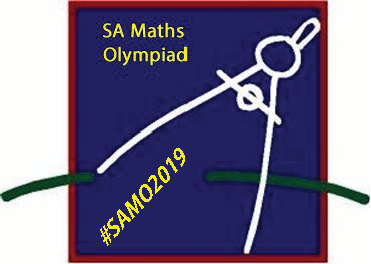
\includegraphics[width=0.18\textwidth]{SAMO2019.png}
\end{tabular} \end{center}


\vspace{30pt}

\begin{center}
\textbf{\Large Senior February Monthly Problem Set}
\\ \vspace{1em}
\textbf{\large Due: 28 February 2018}
\end{center}

\begin{enumerate}[1.]

\item % SW-2013-3
Let $n$ be a positive integer. Both $n$ and $n^2$ only contain the digits $1$, $2$ and $3$ (not necessarily all of them). Determine all possible values of $n$.


\vspace{6pt}
\item % DB-2012-2
Given a (not necessarily convex) quadrilateral $ABCD$, call a point $P$ in the same plane as $ABCD$ an \emph{areal centre} for $ABCD$, if any line through $P$ divides $ABCD$ into two parts of equal area. What are necessary and sufficient conditions on $ABCD$ for it to possess an areal centre?


\vspace{6pt}
\item % The Liam
The (English language version of the) game of Scrabble\texttrademark{} consists of 100 tiles, each containing either a letter from A to Z (some letters occur more than once), except for two blank tiles; see \href{https://en.wikipedia.org/wiki/Scrabble_letter_distributions#English}{\texttt{the relevant Wikipedia page}} for the exact distribution of multiplicities of each letter.

In a solo game of Scrabble, the player starts by choosing seven tiles from the 100 available tiles at random. What is the probability that the player does not pick up any vowels?


\vspace{6pt}
\item % The Robin
For each pair of positive integers $(a, b)$, prove that there exists infinitely many positive integers $n$ such that
$$\frac{a^n + 1}{n^b + 1}$$
is not an integer.


\vspace{6pt}
\item % DB-2012-9
Call a positive integer a \emph{triangular} number if it is of the form $1 +2 +3 +\dotsb +k$ for some positive integer k, and \emph{pentagonal} if it is of the form $1 +4 +7 +10 +13 +\dotsb +(3n-2)$ for some positive integer $n$. Prove that there are infinitely many cases where the product of two consecutive pentagonal numbers is equal to the product of two consecutive triangular numbers.


\vspace{6pt}
\item % Andrew
Let $ABC$ be a triangle with circumcentre $O$. Let $D$ be the point of intersection between the bisector of $\angle ABC$ and the perpendicular bisector of $AB$. Let the circumcircle of $ADO$ be $\omega$. Let $E\neq A$ be the intersection of $\omega$ with the segment $AB$. Let $P\neq E$ be the intersection of the circumcircle of $COE$ with the line $AB$. Prove that $CP$ is tangent to $\omega$.


\vspace{6pt}
\item % Dylan
Call a function $f : \mathbb{N} \to \mathbb{N}$ \emph{almost linear} if $f(m + n) - f(m) - f(n)$ only takes finitely many values as $m$ and $n$ vary through the natural numbers. Suppose that $f : \mathbb{N} \to \mathbb{N}$ and $g : \mathbb{N} \to \mathbb{N}$ are almost linear. Show that $f(g(n)) - g(f(n))$ only takes finitely many values as $n$ varies through the natural numbers.


\vspace{6pt}
\item % Jon
Two people, Alf and Bob, wash up on a desert island. They are greeted by a fearsome monster (Maurice), who challenges them to a game. If they win the monster will show them the way off the island, but if they lose the monster will eat them -- with a nice nutmeg sauce. Seeing little choice they agree to the game (refusing gets them eaten with an avocado sauce). The monster explains the rules. First Maurice will show Alf a standard $8 \times x$ chessboard, on each square of which is a coin, showing either heads or tails. Maurice will then point to a square (so that Alf can see but Bob cannot). No changes are made to the board at this time. Then Alf will play, choosing a single square he will toggle the coin on that square (i.e. change it from heads to tails or from tails to heads). Bob is then shown the adjusted board (the first time Bob gazes on it's wondrousness). Bob must then state which square Maurice chose. If Bob manages to choose the correct square both Alf and Bob go free, but if not... nibbles. Before the game commences Alf and Bob have a chance to discuss their strategy; what is their optimal strategy and how likely are they to escape?


\end{enumerate}

\vfill
\textbf{\Large Email submission guidelines}
\begin{itemize}
	\item Email your solutions to \verb!samf.training.assignments@gmail.com!.
	\item In the subject of your email, include your name and the level of the assignment (Beginner, Intermediate or Senior).
	\item Submit each question in a single separate PDF file (with multiple pages if necessary), with your name and the question number written on each page.
	\item If you take photographs of your work, use a document scanner such as CamScanner to convert to PDF.
	\item If you have multiple PDF files for a question, combine them using software such as PDFsam.
\end{itemize}

\end{document}
